\chapter{Manual de usuario}

Tal y como se especifica en el capítulo 4, la máquina virtual que alberga Jenkins es Ubuntu Server x64 por lo que su manual de usuario e instalación se realizará en base a Ubuntu Server x64 y a Windows 10 como estación de trabajo que alberga la máquina virtual.

En la siguiente dirección se encuentra el repositorio de paquetes de Jenkins para automatizar su instalación \url{https://pkg.jenkins.io/debian-stable/} y actualización. Para poder utilizar este repositorio, primero se debe añadir la clave al sistema:

\begin{console}
$ wget -q -O - https://pkg.jenkins.io/debian-stable/jenkins.io.key | sudo apt-key add -
\end{console}

Después, debemos añadir la siguiente línea al final del archivo /etc/apt/sources.list

\begin{console}
$ deb https://pkg.jenkins.io/debian-stable binary/
\end{console}

Actualizamos los paquetes e instalamos Jenkins.

\begin{console}
$ sudo apt-get update
$ sudo apt-get install jenkins
\end{console}

Una vez que se han realizado estos pasos, obtenemos la dirección IP de la máquina virtual y mediante un navegador web entramos a la dirección IP y al puerto 8080, dicho puerto viene por defecto para Jenkins pero se puede cambiar en la configuración.

\begin{figure}[!h]
\centering
   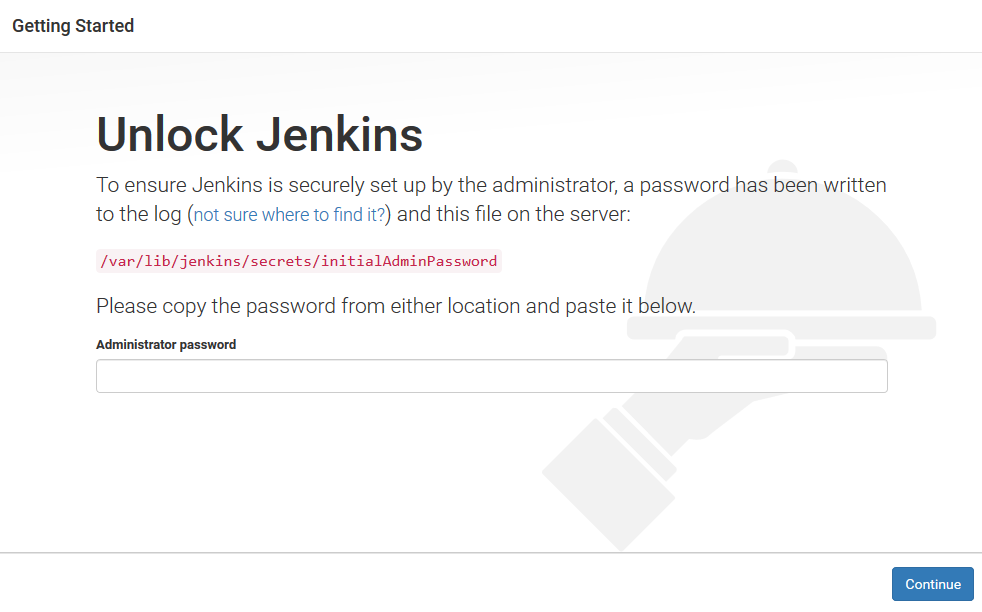
\includegraphics[width=10cm]{PeticionPasswordMaestra.PNG}
\caption{Petición de contraseña maestra de Jenkins}
\end{figure}

\clearpage

Una vez introducimos la contraseña maestra, indicamos los plugins que queremos instalar e indicamos los datos del usuario administrador nos aparece el panel principal de Jenkins vacío listo para comenzar a crear proyectos.

\begin{figure}[!h]
\centering
   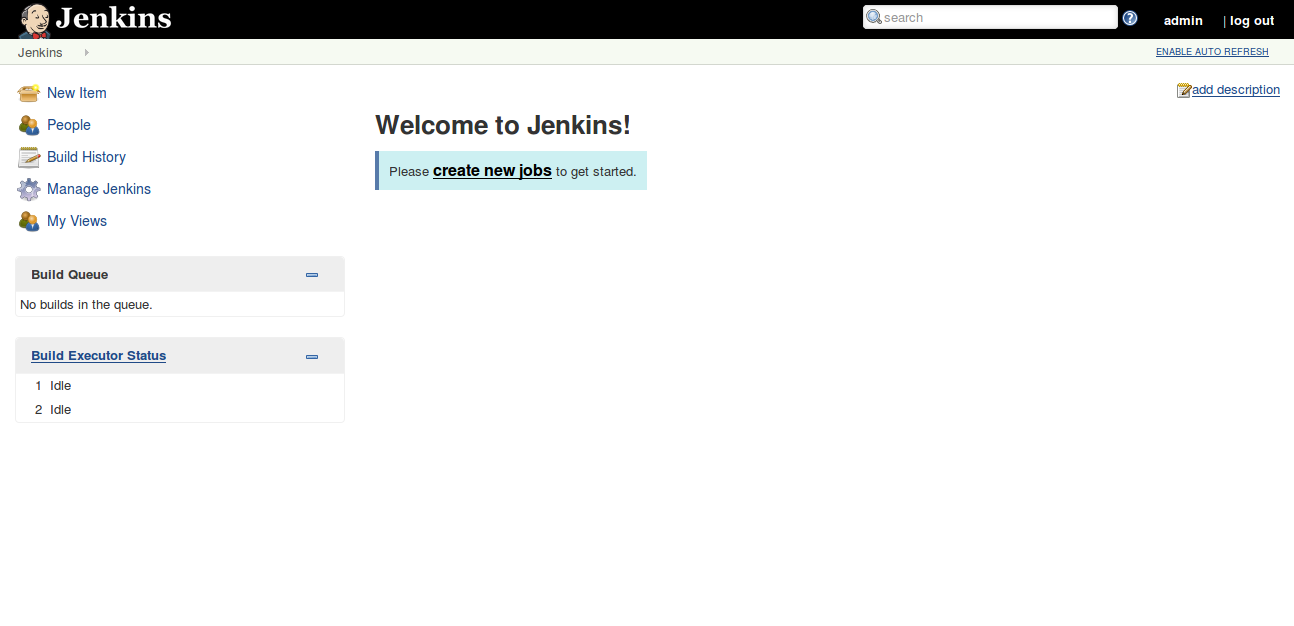
\includegraphics[width=13cm]{JenkinsVacio.png}
\caption{Panel de bienvenida de Jenkins}
\end{figure}

Debido a la posibilidad de poder crear proyectos Maven y compilarlos con Java debemos instalar tanto en la máquina virtual como en el huésped ambas herramientas por lo que para la máquina virtual de Ubuntu Server instalaremos Maven y Java de la siguiente manera:

\begin{console}
$ sudo apt install maven
$ sudo apt install openjdk-8-jdk-headless
\end{console}

En el caso de Windows 10 para Java nos dirigimos a su página oficial, descargamos el archivo e instalamos y de igual manera para Maven, tanto en Ubuntu Server como en Windows 10 se deben configurar las variables de entorno \textit{\$MAVEN\_HOME} y \textit{\$JAVA\_HOME}.

En el caso de Ubuntu Server, sistema operativo donde se alberga Jenkins, hay que indicarle la ruta de ambas variables para su correcta configuración, además de la ruta donde está instalado Git, sistema de control de versiones utilizado.

\begin{figure}[!h]
\centering
   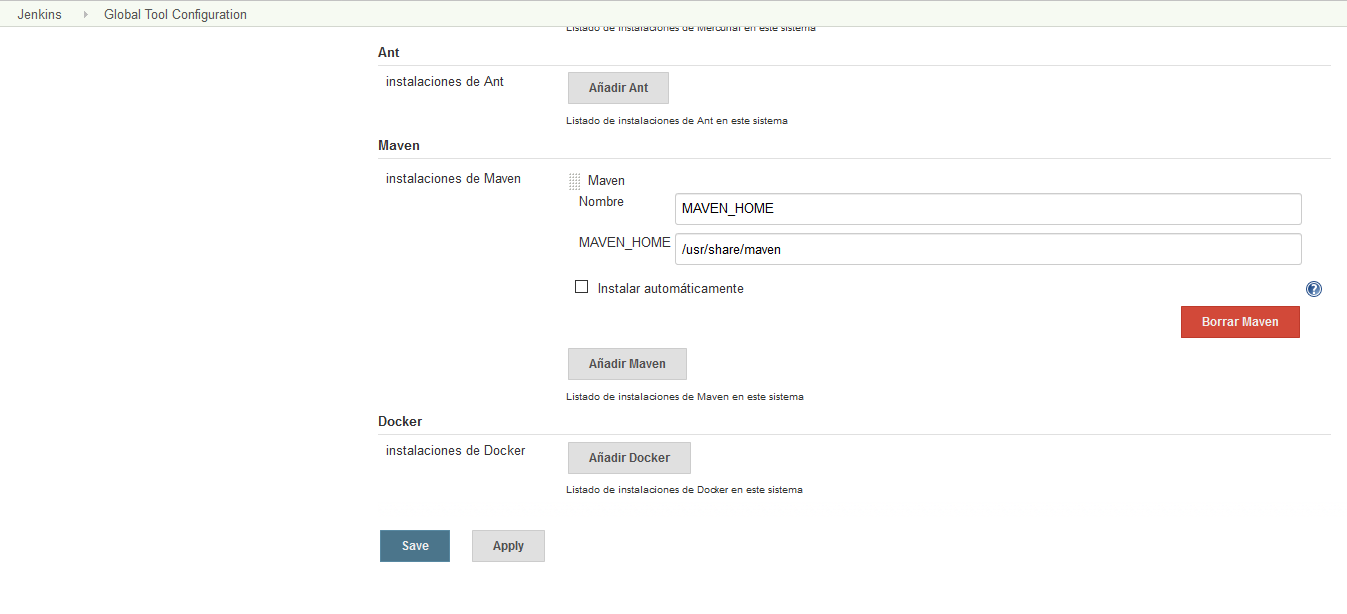
\includegraphics[width=12cm]{ParametroMAVENHOME.PNG}
\caption{Parámetros de configuración de Jenkins}
\end{figure}

\clearpage

Con la configuración actual, podemos realizar ejecuciones en local, es decir, en Ubuntu Server pero lo que queremos para realizar el sistema de integración continua de manera correcta, es que Ubuntu Server sea el orquestador y se realicen las ejecuciones en otros computadores esclavos, por lo que ahora vamos a crear un esclavo con la configuración de Windows 10, al cual debemos indicarle la información dicha anteriormente.

\begin{figure}[!h]
\centering
   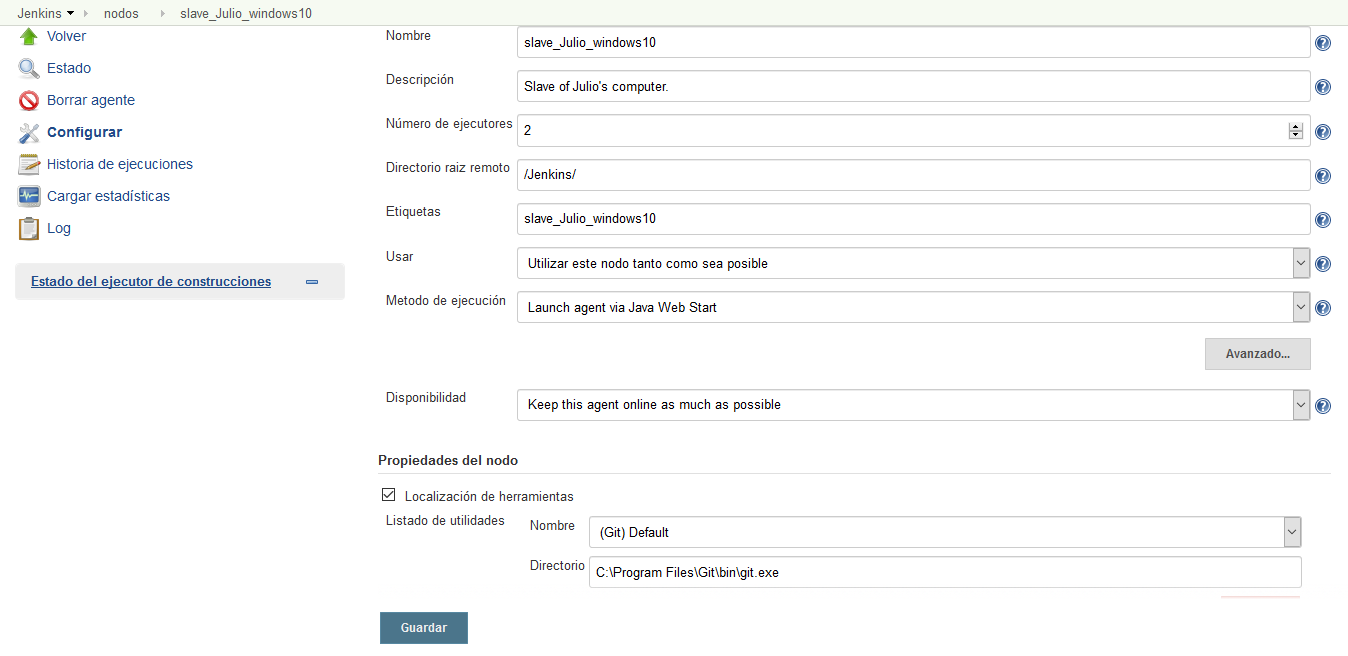
\includegraphics[width=12cm]{ParametroEsclavo.PNG}
\caption{Parámetros de configuración de un esclavo Jenkins}
\end{figure}

Una vez realizada esta instalación, podemos crear un proyecto en Jenkins, en este caso un proyecto Maven, donde indicamos la dirección del repositorio donde se encuentra el proyecto para que lo instale, el esclavo donde se va a realizar la ejecución, proyectos padres, las acciones anteriores y posteriores que se deben realizar en la ejecución...

\begin{figure}[!h]
\centering
   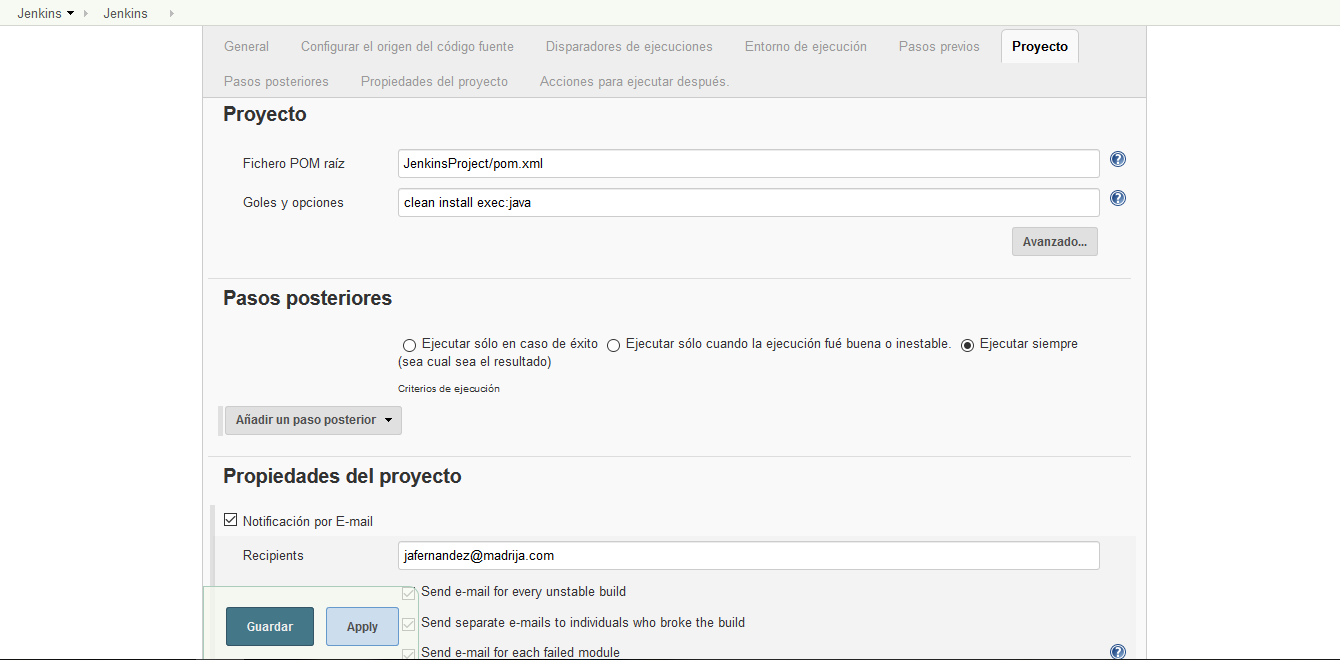
\includegraphics[width=12cm]{ParametroProyectoJenkins.PNG}
\caption{Configuración de un proyecto Jenkins}
\end{figure}

\clearpage

Una vez realizadas todas las configuraciones necesarias, se puede ejecutar el proyecto y obtener los resultados de su ejecución.

\begin{figure}[!h]
\centering
   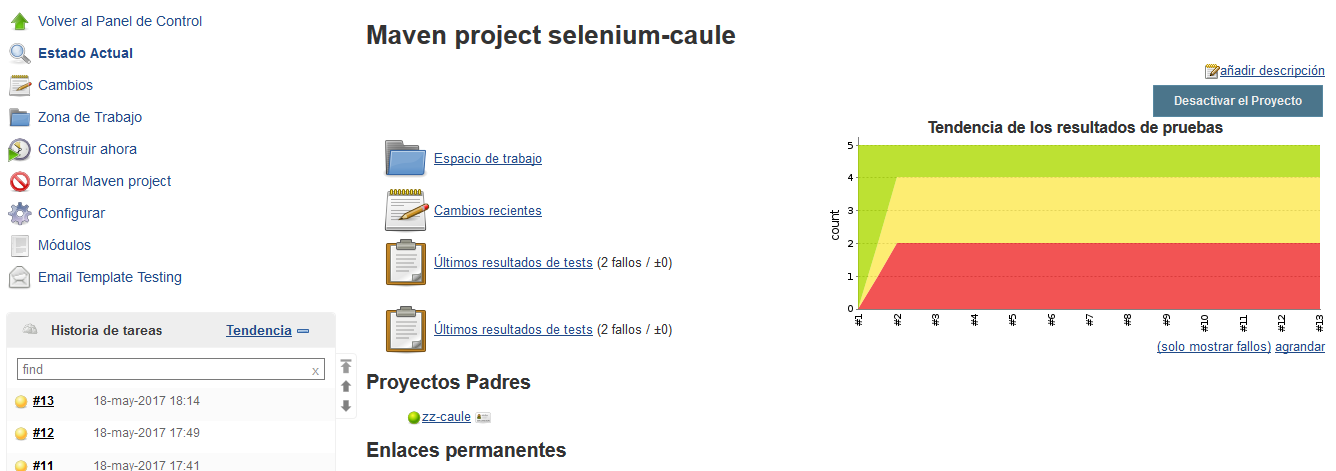
\includegraphics[width=14cm]{ResultadosJenkins.PNG}
\caption{Resultados tras ejecutar un proyecto Jenkins}
\end{figure}
